\documentclass[11pt,a4paper]{article}
\usepackage[margin=2.3cm]{geometry}
\usepackage[T1]{fontenc}
\usepackage{lmodern}
\usepackage{amsmath,amssymb,amsthm}
\usepackage{graphicx}
\usepackage{booktabs}
\usepackage{hyperref}
\usepackage{xcolor}
\renewcommand{\topfraction}{0.9}\renewcommand{\textfraction}{0.1}\renewcommand{\floatpagefraction}{0.8}

\hypersetup{colorlinks=true,linkcolor=blue!50!black,citecolor=blue!50!black,urlcolor=blue!50!black}
\newtheorem{proposition}{Proposition}
\newcommand{\E}{\mathbb{E}}
\newcommand{\Var}{\mathrm{Var}}
\newcommand{\nlive}{n_{\mathrm{live}}}
\newcommand{\code}[1]{\texttt{#1}}

\title{When to retrain the flow in \textsc{nessai}:\\ a renewal-theory decision model}
\author{Investigation notes, branch \code{claude/nessai-retrain-decision-pmm9kr}}
\date{\today}

\begin{document}
\maketitle

\begin{abstract}
We build a simple, principled rule for deciding, before each nested-sampling
iteration, whether to retrain (or reset) the normalising flow in
\textsc{nessai}, with the aim of minimising total run time. Instrumented runs
show that (i) the proposal pool is paid for when it is populated, so the only
sensible decision points are when the pool is empty, and (ii) between
trainings the acceptance decays as $\exp(-s/\nlive)$ with remarkable
precision. Under these facts the problem is a classic renewal
(machine-replacement) problem. It has a closed-form optimal long-run cost rate
$g^*$, which answers the question of how far ahead to look: one training
cycle, with everything beyond it summarised by $g^*$. The rule is to retrain
when the next pool drawn from the current flow would cost more per iteration
than $g^*$. Uncertainties are propagated at the Gaussian level and calibrated
on the run's own history. Costs are deterministic counts multiplied by unit
costs, which are either provided by the user (deterministic schedule) or
measured. On three test problems with six seeds each, the rule reduces run time
relative to \textsc{nessai}'s default schedule by 16\% when training dominates
the cost and by 17\% when the likelihood dominates (emulated
$t_L=10\,ms$). In between it is neutral, and it is never significantly
worse. A fixed schedule is up to $1.6\times$ slower. The reset option gains a
further 12\% at $t_L=10\,ms$, coming mostly from the bimodal problem.
\end{abstract}

\section{Setting and empirical facts}\label{sec:facts}

In \textsc{nessai}'s standard nested sampler a pool of $P$ points is drawn
from the flow proposal. All $P$ likelihoods are evaluated when the pool is
populated, and each iteration then draws points from the pool until one lies
above the current likelihood contour. Let
\begin{itemize}
  \item $c$ be the cost of one pool point (flow sampling, rejection sampling,
        likelihood evaluation, amortised loop overhead);
  \item $T$ be the cost of training the flow;
  \item $a(s)$ be the acceptance $s$ iterations after the last training, i.e.\
        the probability that a pool point lies inside the current contour.
\end{itemize}
Each iteration consumes on average $1/a$ pool points, so the cost per
iteration is $r(s)=c/a(s)$.

\paragraph{Fact 1: the pool is paid up front.} \code{FlowProposal.train}
discards the current pool. Retraining with a non-empty pool therefore throws
away points whose cost has already been paid, while using up the pool costs
(almost) nothing extra. Retrain decisions should only be taken when the pool
is empty. Fixed-frequency schedules violate this: \code{training\_frequency=500}
with \code{train\_on\_empty=False} used 1.1--1.6$\times$ the likelihood
evaluations of the default (train-on-empty) schedule, for a similar number
of trainings.

\paragraph{Fact 2: exponential decay at a known rate.} If the flow density
$q$ is approximately constant over the region enclosed by the contour, the
acceptance is $a=\int_{L>L^*}q\,\mathrm{d}\theta\approx\bar q\,X$. The prior
volume shrinks as $X\propto e^{-i/\nlive}$, so
\begin{equation}
  a(s) = A\,e^{-k s},\qquad k \simeq 1/\nlive, \label{eq:decay}
\end{equation}
where $A$ is the ``fresh'' acceptance of the newly trained flow.
Figure~\ref{fig:decay} shows episodes of 3000 iterations without retraining
on three problems. The fitted slopes are $k\nlive=1.00\pm0.04$, the linear
model fits to within the counting noise, and the result holds even at the
start of an episode. The exponential model is therefore exact in practice
and the rate is known a priori. We still fit it, with a prior centred on
$1/\nlive$, because proposal schemes that shrink the proposal volume between
trainings would change it.

\begin{figure}[htbp]
  \centering
  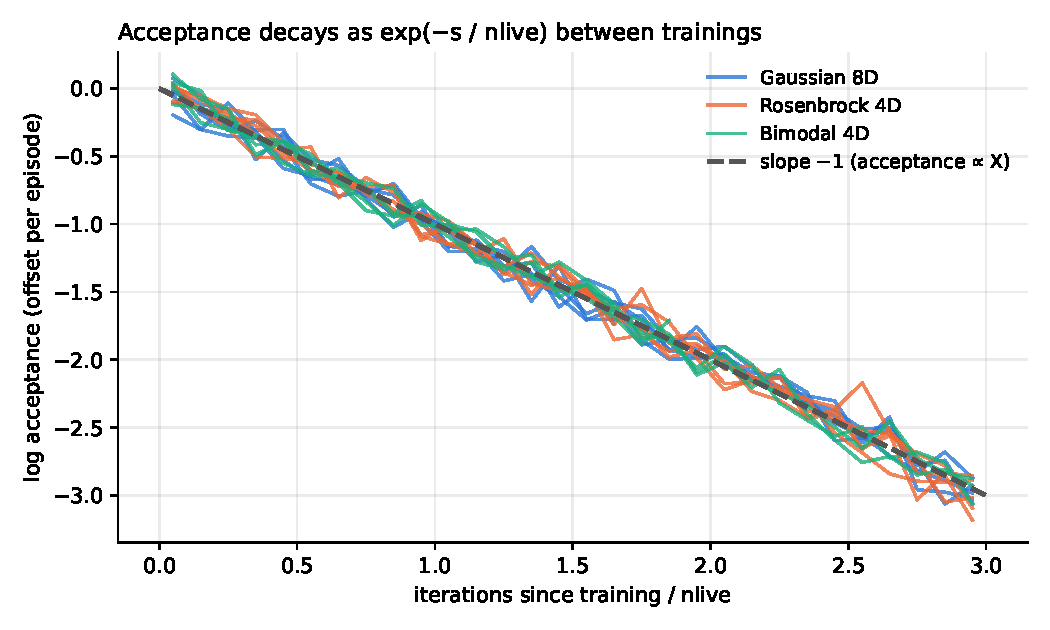
\includegraphics[width=0.62\textwidth]{fig_decay.pdf}
  \caption{Binned log-acceptance in episodes of 3000 iterations between
  trainings ($\nlive=1000$). The dashed line has slope $-1/\nlive$.}
  \label{fig:decay}
\end{figure}

\paragraph{Fact 3: the fresh acceptance is a level, not a gain.} The fresh
acceptance $A$ of a warm-started retrain does not depend on how long ago the
previous training was, so a multiplicative ``improvement''
$A_{\rm new}/a_{\rm before}$ is not a stable quantity (it grows as
$e^{k\,\mathrm{gap}}$). We therefore predict $\log A$ as a level estimated
from recent episodes. It drifts slowly over the run, in either direction.

\paragraph{Fact 4: training cost.} The time per epoch is very stable, and the
number of epochs of a warm start grows mildly with the gap (about 30 at
500-iteration gaps vs.\ about 100 at 3000 on Rosenbrock/bimodal). A full reset
costs 3--5$\times$ the epochs of a warm start.

\section{The decision model}

\subsection{How far to look ahead}

Consider two policies at a moment when the pool is empty:
\begin{itemize}
  \item[(R)] retrain now, then act optimally;
  \item[(C)] draw one more pool of $P$ points from the current flow, lasting
        $n$ iterations, then retrain and act optimally.
\end{itemize}
The number of iterations $N$ of a run is set by the stopping criterion, not by
the schedule. After the extra block, (C) therefore follows the same process as
(R), shifted by $n$ iterations. If the long-run cost per iteration of the
optimal schedule is $g^*$, then
\begin{equation}
  \mathrm{Cost}(C)-\mathrm{Cost}(R) \;\longrightarrow\; cP - g^*\,n
  \label{eq:diff}
\end{equation}
as the remaining horizon grows. This is the constant to which the two
exponentially growing cost curves converge. They only cancel if future
retraining is allowed in both branches; if it is not, both costs diverge and
their difference is dominated by the better flow, which always favours
retraining. Equation~\eqref{eq:diff} gives the rule
\begin{equation}
  \boxed{\text{retrain} \iff c\,P > g^*\,\E[n]}
  \label{eq:rule}
\end{equation}
i.e.\ retrain when continuing costs more per iteration than the optimal
long-run rate. The effective horizon is one training cycle.

\subsection{The optimal long-run rate}

A cycle that starts with a training and lasts $\tau$ iterations costs
\begin{equation}
  C(\tau) = T + \int_0^\tau \frac{c}{A'}e^{ks}\,\mathrm{d}s
          = T + \frac{c}{A'k}\left(e^{k\tau}-1\right),
\end{equation}
where $A'$ is the fresh acceptance of the next flow. By the renewal-reward
theorem the long-run cost per iteration is $g(\tau)=C(\tau)/\tau$.

\begin{proposition}
Let $y = TkA'/c$ (the training cost in units of the cost of $1/k$ iterations
of a fresh flow). The minimum $g^*=\min_\tau g(\tau)$ is $g^* = x\,c/A'$,
reached at $\tau^* = \ln(x)/k$, where $x\geq1$ is the unique solution of
\begin{equation}
  x\ln x - x + 1 = y. \label{eq:renewal}
\end{equation}
Equivalently, $g^*$ satisfies
\begin{equation}
  T = \int_0^\infty \left(g^* - \frac{c}{A'}e^{ks}\right)^+ \mathrm{d}s .
  \label{eq:savings}
\end{equation}
\end{proposition}
\begin{proof}
$g'(\tau)=0 \iff \tau\,C'(\tau) = C(\tau)$. Since $C'(\tau) = c e^{k\tau}/A'$,
at the optimum the instantaneous rate equals the average rate:
$c e^{k\tau^*}/A' = g^*$. Writing $x=e^{k\tau^*}$, the condition
$C(\tau^*) = g^*\tau^*$ becomes
$T + \frac{c}{A'k}(x-1) = \frac{c}{A'}x\frac{\ln x}{k}$, which is
\eqref{eq:renewal}. The left-hand side of \eqref{eq:renewal} is increasing
for $x>1$ and vanishes at $x=1$, so the solution is unique. For
\eqref{eq:savings}, $\int_0^{\tau^*}(g^*-c e^{ks}/A')\,\mathrm{d}s
= g^*\tau^* - (C(\tau^*)-T) = T$.
\end{proof}

Equation~\eqref{eq:savings} has a simple reading: the training cost is
recovered by the savings accumulated while the new flow runs below the
break-even rate (Fig.~\ref{fig:schematic}). Limits:
\begin{equation}
  y\ll1:\quad x\simeq 1+\sqrt{2y},\;\;
  \tau^*\simeq\sqrt{\frac{2T A'\nlive}{c}};
  \qquad
  y\gg1:\quad x\simeq \frac{y}{\ln y}.
\end{equation}
The small-$y$ limit is a square-root law, analogous to the economic order
quantity. Equation~\eqref{eq:renewal} is solved by bisection.

\begin{figure}[htbp]
  \centering
  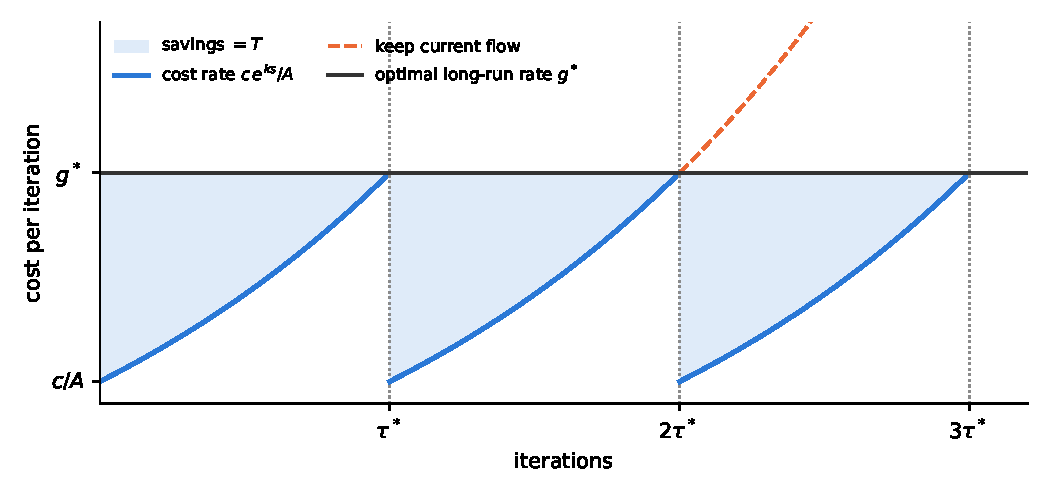
\includegraphics[width=0.72\textwidth]{fig_schematic.pdf}
  \caption{Cost per iteration under the optimal policy. Each shaded area
  equals $T$; keeping the current flow past $\tau^*$ (dashed) costs more
  than $g^*$ per iteration.}
  \label{fig:schematic}
\end{figure}

\paragraph{Training cost growing with the gap.} If $T=T_0+T_1\tau$, then
$g(\tau) = T_1 + [T_0 + \tfrac{c}{A'k}(e^{k\tau}-1)]/\tau$, and in
\eqref{eq:rule} continuing for $n$ iterations also adds $T_1 n$ to the next
training. $T_1$ cancels, so only the fixed part $T_0$ matters. Using the mean
training cost (as we do) slightly overestimates $T_0$ and is mildly
conservative.

\subsection{Pool yield, pool planning and finite horizon}

\paragraph{Yield.} A pool of $P$ points drawn $s$ iterations after training
lasts $n$ iterations, where $\int_s^{s+n} e^{ks'}\mathrm{d}s'/A = P$, i.e.
\begin{equation}
  n = \frac{1}{k}\ln\!\left(1 + P k\,a(s)\right).
\end{equation}
With \textsc{nessai}'s default pool size $P\approx\nlive/\bar a$ a pool lasts
roughly $0.3$--$0.7\,\nlive$ iterations.

\paragraph{Pool planning.} Since decisions happen when the pool is empty, the
schedule cannot retrain more often than once per pool. When $\tau^*$ is
shorter than a pool (expensive likelihoods), we cap the next pool at the
number of points needed to reach the break-even point
$c/a(s')=g^*$:
\begin{equation}
  P_{\rm plan} = \frac{1}{k}\left(\frac{g^*}{c} - \frac{1}{a(s)}\right),
\end{equation}
with a floor corresponding to $\max(\nlive/10, \text{bin size})$ iterations.
After a retrain the same formula is used with $a=A'$. There is no penalty for
smaller pools beyond a small fixed overhead per population.

\paragraph{Finite horizon.} We estimate the remaining iterations from the
stopping criterion. With $\Delta\log Z = \log(1+L_{\max}X/Z)$ and
$X\propto e^{-i/\nlive}$,
$N_{\rm rem}\simeq\nlive[\log(e^{\Delta\log Z}-1)-\log(e^{\epsilon}-1)]$.
If $N_{\rm rem}<\tau^*$ we compare the expected costs to the end directly,
without further retraining:
$T + \frac{c}{A'k}(e^{kN_{\rm rem}}-1)$ against
$\frac{c}{a(s)k}(e^{kN_{\rm rem}}-1)$.

\subsection{Resetting the flow}

A reset replaces warm-start training by training from scratch, with cost
$T_{\rm r}$ and fresh acceptance $A_{\rm r}$. We model
$\log A_{\rm r} = \log A_{\rm w} + \delta$ and compute $g^*_{\rm r}$ from
\eqref{eq:renewal} with $(T_{\rm r}, A_{\rm r})$. When retraining, we reset
if $g^*_{\rm r}<g^*_{\rm w}$. The posterior on $\delta$ is Gaussian, combining
a prior $\mathcal N(0,1)$ with two kinds of evidence:
\begin{itemize}
  \item \emph{lineage degradation}: $\log A$ of the first (from-scratch)
        episode of the current lineage minus the current warm prediction, with
        variance $\sigma_0^2 + (\gamma\,\Delta i/\nlive)^2$. Its relevance
        decays as the posterior changes ($\sigma_0=0.3$, $\gamma=0.05$);
  \item \emph{paired outcomes of past resets}: $\log A$ of each reset episode
        minus that of the preceding episode, with variance $2\sigma_0^2$.
\end{itemize}
A lineage that has degraded since it started favours a reset; a lineage that
has improved, or a reset that did not help, counts against one. With no
evidence, $\E[\delta]=0$ and the larger $T_{\rm r}$ prevents resets.

\section{Estimating the inputs with uncertainties}

\paragraph{Current flow.} The draws needed per iteration are geometric,
$m_i\sim\mathrm{Geom}(a_i)$. Binning $b$ iterations gives
$\hat a = b/\sum m_i$ with, by the delta method,
\begin{equation}
  \Var[\log\hat a]\simeq \frac{1-a}{b}.
\end{equation}
We fit $\log a(s)=\alpha+\beta s$ by weighted least squares with a conjugate
Gaussian prior, which gives a closed-form Gaussian posterior on
$(\alpha,\beta)$. The prior on $\alpha$ is the fresh-level prediction below,
and the prior on $\beta$ is the precision-weighted mean of recent episodes
(initially $-1/\nlive\pm30\%$). The bin size is $\max(10,\nlive/20)$.

\paragraph{Fresh flow.} For every finished episode we store a data-only fit
$\widehat{\log A}_j$. The prediction for the next warm retrain is the mean of
the last $m=5$ episodes of the current lineage. Its predictive variance is
calibrated on the run's own past prediction errors $e_j$:
\begin{equation}
  \sigma^2_{A'} = \frac{w_0\sigma_p^2 + \sum_j e_j^2}{w_0 + N_e},
  \qquad \sigma_p = 0.3,\; w_0=2 .
\end{equation}
This replaced a sample variance over the last five episodes, whose error bars
were too narrow (Table~\ref{tab:calib}).

\paragraph{Propagation.} Costs are convex in $1/a$, so uncertainties raise
expected costs through log-normal moments:
\begin{equation}
  \E[1/A'] = e^{-\mu+\sigma^2/2},\qquad
  \E[1/k]\simeq \frac{1}{\hat k}\left(1+\frac{\sigma_k^2}{\hat k^2}\right),
\end{equation}
which enter \eqref{eq:renewal} through $A_{\rm eff}=1/\E[1/A']$ and
$k_{\rm eff}=1/\E[1/k]$. $\E[n]$ is computed by 7-point Gauss--Hermite
quadrature over the posterior of $\log a(s)$. $c$ and $T$ enter linearly, so
only their means affect the expected cost.

\begin{table}[htbp]
\centering
\caption{Calibration of the Gaussian predictions (z-scores; the ideal is mean
0, sd 1 and 4.6\% beyond $2\sigma$).}
\label{tab:calib}
\begin{tabular}{lrrrr}
\toprule
prediction & $N$ & mean $z$ & sd $z$ & $|z|>2$ \\
\midrule
$\log a$ at the start of the next pool & 648 & $-0.06$ & 1.03 & 5.2\% \\
pool yield $n$ (log ratio realised/predicted) & 648 & \multicolumn{3}{l}{bias $-2\%$, scatter 7\%} \\
fresh $\log A'$, sample variance of 5 episodes & 727 & $-0.4\ldots+0.3$ & 1.2--1.8 & 15--24\% \\
fresh $\log A'$, calibrated variance & 727 & $-0.2\ldots+0.2$ & 0.87--1.12 & 3.4--6.5\% \\
\bottomrule
\end{tabular}
\end{table}

\section{Costs and determinism}

All costs are deterministic counts multiplied by three unit costs:
likelihood evaluations $\times$ [s/evaluation], pool points $\times$
[s/point], and epochs $\times$ training samples $\times$ [s/(sample$\cdot$epoch)].
For a fixed seed the epoch counts are deterministic, since early stopping
depends only on the data and the seed. With
\code{retrain\_costs=dict(likelihood=..., population=..., training=...)}, or
the path of a previous run's \code{retrain\_costs.json}, the schedule is
fully deterministic. In the benchmark, decision runs whose costs make them
retrain at every empty pool reproduced the default schedule's trajectory
exactly. Missing unit costs are measured during the run, which makes the
schedule depend on the hardware. Measured costs are always tracked:
\begin{itemize}
  \item likelihood time comes from the model's counters;
  \item population cost is the non-training sampling time minus likelihood
        time, per pool point;
  \item training cost is the wall time per sample-epoch.
\end{itemize}
A warning is logged if a measured cost differs from the provided value by
more than $2\times$ (after three measurements), and the measured costs are
written to \code{retrain\_costs.json} at the end of the run.

\section{Experiments}

\paragraph{Setup.} Three problems: an 8D Gaussian, 4D Rosenbrock and a 4D
bimodal correlated Gaussian. $\nlive=1000$, the default \code{FlowProposal},
and a flow with 4 blocks of 2$\times$16 neurons; CPU, one thread per run.
The test likelihoods are nearly free (0.1\,$\mu$s), so we
emulate expensive ones with a \emph{virtual} cost $t_L$:
\[
  \text{virtual time} = \text{wall time} + N_{\rm like}\,t_L,
  \qquad t_L\in\{0, 10^{-4}, 10^{-3}, 10^{-2}\}\,\mathrm{s}.
\]
Decision runs receive $t_L$ through \code{retrain\_costs}, together with the
measured unit costs for population (75\,$\mu$s/point) and
training (14\,$\mu$s/sample-epoch). The dimensionless training
cost $y$ spans about 2 ($t_L=0$) down to about 0.015 ($t_L=10^{-2}$), and
$\tau^*$ spans about $1.3\nlive$ down to $0.16\nlive$. Policies:
\begin{itemize}
  \item \emph{default}: train on empty, cooldown 200, retrain when acceptance
        $<0.01$;
  \item \emph{fixed}: every 1000 iterations;
  \item \emph{decision}: rule \eqref{eq:rule} with pool planning, with
        provided costs, or with measured costs (\emph{dyn});
  \item \emph{decision + reset}.
\end{itemize}
Each (problem, policy, $t_L$) is run with 6 seeds. Comparisons are paired by
problem and seed and summarised by the geometric mean of the time ratio to
\emph{default}, with a 95\% bootstrap interval.

\subsection{Results}

\begin{table}[htbp]\centering
\caption{Run time relative to the default schedule (geometric mean over 3 problems $\times$ 6 seeds, 95\% bootstrap interval), mean number of trainings and resets.}
\label{tab:results}
\begin{tabular}{llcrr}
\toprule
$t_L$ [s] & policy & time ratio & trainings & resets \\
\midrule
0 & default & 1 & 27.3 & 0 \\
 & fixed (1000 it) & 0.88 [0.83, 0.93] & 14.8 & 0.0 \\
 & decision & 0.84 [0.78, 0.90] & 11.0 & 0.0 \\
 & decision (measured costs) & 0.82 [0.77, 0.88] & 11.2 & 0.0 \\
 & decision + reset & 0.85 [0.79, 0.91] & 10.5 & 0.8 \\
\midrule
0.0001 & default & 1 & 27.3 & 0 \\
 & fixed (1000 it) & 1.05 [1.01, 1.08] & 14.8 & 0.0 \\
 & decision & 0.94 [0.90, 0.98] & 14.9 & 0.0 \\
 & decision + reset & 0.95 [0.88, 1.01] & 13.9 & 0.7 \\
\midrule
0.001 & default & 1 & 27.3 & 0 \\
 & fixed (1000 it) & 1.41 [1.34, 1.47] & 14.8 & 0.0 \\
 & decision & 0.99 [0.94, 1.04] & 26.1 & 0.0 \\
 & decision + reset & 0.92 [0.81, 1.03] & 24.1 & 0.8 \\
\midrule
0.01 & default & 1 & 27.3 & 0 \\
 & fixed (1000 it) & 1.57 [1.48, 1.65] & 14.8 & 0.0 \\
 & decision & 0.83 [0.78, 0.87] & 59.5 & 0.0 \\
 & decision + reset & 0.73 [0.63, 0.84] & 55.3 & 1.2 \\
\bottomrule
\end{tabular}
\end{table}
\begin{table}[htbp]\centering
\caption{Time ratio to default per problem (geometric mean over 6 seeds).}
\label{tab:perproblem}
\begin{tabular}{llccc}
\toprule
$t_L$ [s] & policy & Gaussian 8D & Rosenbrock 4D & bimodal 4D \\
\midrule
0 & decision & 0.90 & 0.86 & 0.77 \\
0 & decision + reset & 0.90 & 0.87 & 0.79 \\
0 & fixed (1000 it) & 0.86 & 0.94 & 0.84 \\
0.0001 & decision & 1.00 & 0.91 & 0.91 \\
0.0001 & decision + reset & 1.00 & 0.97 & 0.89 \\
0.0001 & fixed (1000 it) & 1.07 & 1.06 & 1.01 \\
0.001 & decision & 0.92 & 1.07 & 0.98 \\
0.001 & decision + reset & 0.97 & 0.98 & 0.83 \\
0.001 & fixed (1000 it) & 1.48 & 1.39 & 1.35 \\
0.01 & decision & 0.74 & 0.90 & 0.85 \\
0.01 & decision + reset & 0.79 & 0.81 & 0.62 \\
0.01 & fixed (1000 it) & 1.64 & 1.58 & 1.49 \\
\bottomrule
\end{tabular}
\end{table}

\begin{figure}[htbp]
  \centering
  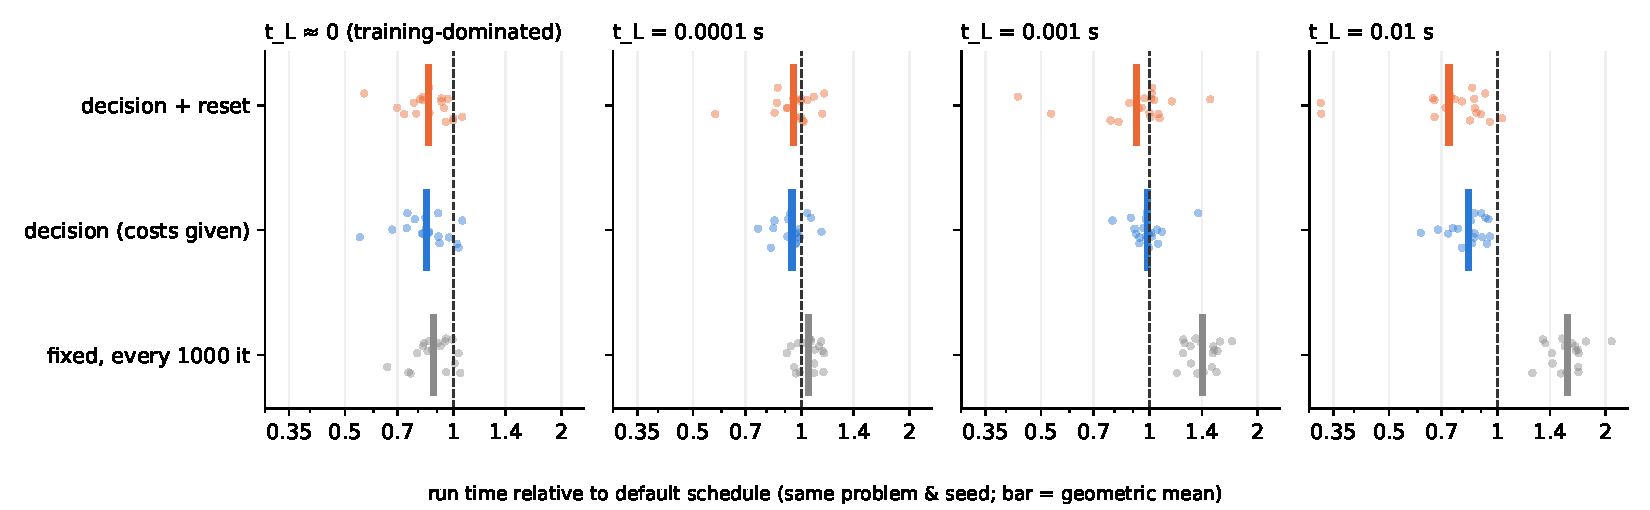
\includegraphics[width=\textwidth]{fig_compare.pdf}
  \caption{Run time of each run relative to the default schedule on the same
  problem and seed (dots), with the geometric mean (bars). Panels are for
  increasing emulated likelihood cost.}
  \label{fig:compare}
\end{figure}

Tables~\ref{tab:results} and~\ref{tab:perproblem} and Fig.~\ref{fig:compare}
show the following.
\begin{itemize}
  \item \textbf{Training-dominated regime} ($t_L\approx0$, $y\approx2$):
        the decision takes $0.84\,[0.78, 0.90]$ of the default's time. It
        trains 11 times instead of 27, with $\tau^*\approx1.3\nlive$.
        Measuring the costs during the run instead of providing them gives
        the same result ($0.82$).
  \item \textbf{Intermediate regime} ($t_L=10^{-4}$, $10^{-3}$\,s):
        $0.94\,[0.90,0.99]$ and $0.99\,[0.94,1.04]$. Here $\tau^*$ is close to
        the default pool length (0.3--0.7$\nlive$), so the default
        train-on-empty schedule happens to be near-optimal and there is little
        to gain.
  \item \textbf{Likelihood-dominated regime} ($t_L=10^{-2}$\,s, $y\approx0.015$):
        $0.83\,[0.78, 0.87]$. $\tau^*\approx0.16\nlive$ is shorter than a pool,
        and pool planning lets the rule retrain about 60 times instead of 27.
        Without pool planning (earlier batch) the rule matched the default
        exactly: it retrained at every empty pool and reproduced the default
        trajectory.
  \item \textbf{Fixed schedules} discard partially used pools. Every 1000
        iterations is competitive only when training dominates, and costs
        $1.41$--$1.57\times$ the default when likelihoods are expensive.
  \item \textbf{Reset.} The reset option triggers 0.7--1.2 times per run. It is
        neutral on the unimodal problems and helps on the bimodal one, where
        warm-started lineages sometimes degrade ($0.62$ vs.\ $0.85$ for the
        plain decision at $t_L=10^{-2}$; $0.83$ vs.\ $0.98$ at $10^{-3}$).
        Overall, $0.73\,[0.63,0.84]$ at $t_L=10^{-2}$ and consistent with
        the plain decision elsewhere. Resets pay off more when the likelihood
        is expensive, because the gain in acceptance is then worth more than
        the 3--5$\times$ higher training cost.
  \item \textbf{Evidence.} $\log Z$ is unaffected. For the Gaussian, all
        policies give $-16.61\pm0.10$ (analytic $-16.614$); for the bimodal,
        $-10.59\pm0.09$ (analytic $-10.604$), with the same scatter as the
        default.
\end{itemize}

\section{Discussion and limitations}

\begin{itemize}
  \item \textbf{Test problems.} The benchmark problems are small, and
        training dominates wall time unless $t_L$ is large. The structure of
        the rule does not depend on this, since everything enters through
        $y=TkA'/c$. Confirming the gains on production problems (e.g.\ GW
        likelihoods with the group-mixture flows of this fork) is the obvious
        next step.
  \item \textbf{Trajectory noise.} Seed-to-seed variance is large. Warm-start
        lineages can drift to a 3$\times$ different likelihood count on the
        same problem, which dominates single-run comparisons.
  \item \textbf{Pool granularity.} Without pool planning the rule can only
        choose among multiples of the pool length, and for expensive
        likelihoods it cannot improve on the default.
  \item \textbf{Resetting} is an exploration problem: we only learn what a
        reset gives by resetting. The lineage-relative evidence avoids the
        worst failure (repeatedly resetting into worse flows), but its prior
        parameters ($\sigma_0$, $\gamma$) are set by hand from a handful of
        runs.
  \item \textbf{Model assumptions.} Training outcomes are treated as
        independent of the gap, apart from the mean cost, and the future is
        assumed stationary within one cycle; slow drifts are tracked by
        re-estimating at every decision. The population unit cost absorbs the
        per-iteration loop overhead.
\end{itemize}

\paragraph{Usage.}
\begin{verbatim}
FlowSampler(model, ...,
            retrain_decision=True,          # or dict(allow_reset=True, ...)
            retrain_costs="previous_run/retrain_costs.json")
\end{verbatim}
Code: \code{src/nessai/samplers/retrain.py}. Experiments and scripts:
\code{examples/retrain\_decision/}.

\end{document}
